\begin{frame}
\frametitle{Inertial particles and turbulence}
	% Applications
%    \begin{textblock*}{90mm}[0,0](-5mm,-2mm)
%    \textcolor{myred}{\textbf{Many fields of application}}
%    \begin{itemize}
%        \item \textbf{Natural} : plankton, marine snow, rain, pollutants
%        \item \textbf{Industrial} : chemical reactors, combustion chambers
%    \end{itemize}
%    \end{textblock*}
    
\begin{textblock*}{30mm}[0,0](0mm,2mm)
	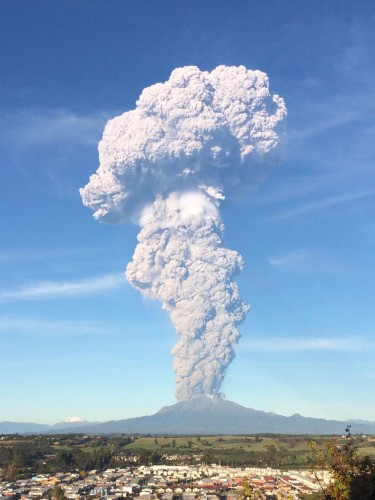
\includegraphics[width = \textwidth]{volcano.jpg}
\end{textblock*}
\begin{textblock*}{45mm}[0,0](0mm,45mm)
{\footnotesize Aerosol and climate forcing\\
Aviation safety\\
}\end{textblock*}

\begin{textblock*}{35mm}[0,0](42mm,-1mm)
	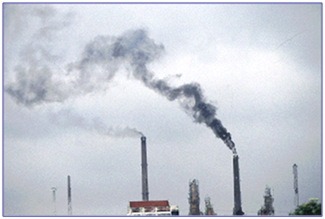
\includegraphics[width = \textwidth]{Cheminees.png}
\end{textblock*}
\begin{textblock*}{35mm}[0,0](40mm,30mm)
	\centering
\textcolor{myred}{{\textbf{Settling alteration\\-\\Dispersion}}}
\end{textblock*}
\begin{textblock*}{30mm}[0,0](5mm,55mm)
	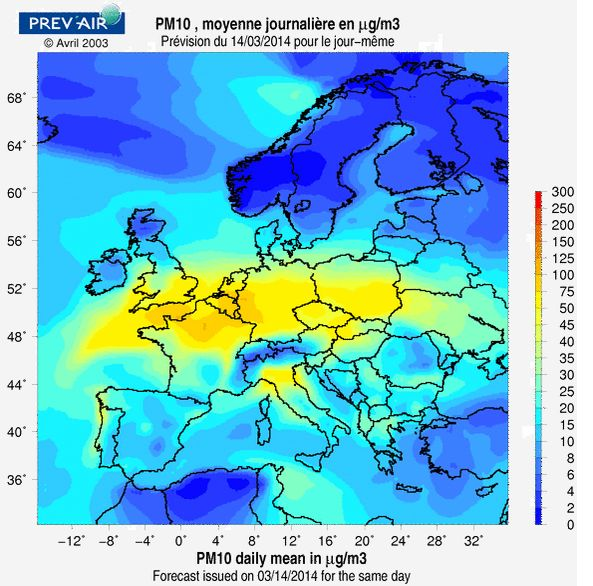
\includegraphics[clip,trim=30 45 58 55,width = \textwidth]{Carte_PM10_Europe_20140314.JPG}
\end{textblock*}


\begin{textblock*}{30mm}[0,0](83mm,0mm)
	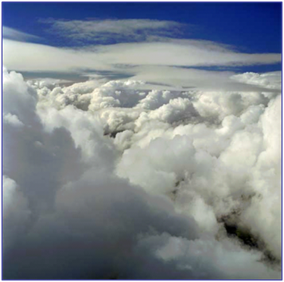
\includegraphics[width = \textwidth]{Nuages.png}\\
	\footnotesize{Rain formation alteration}
\end{textblock*}
\begin{textblock*}{30mm}[0,0](83mm,43mm)
	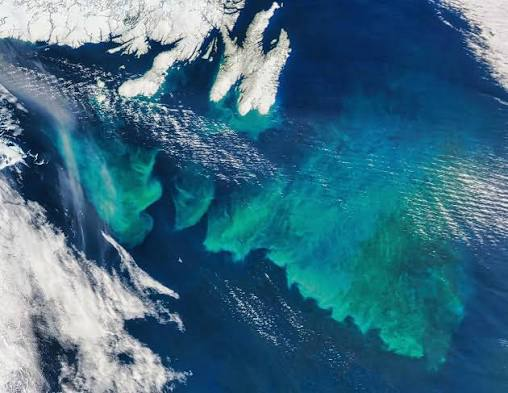
\includegraphics[width = \textwidth]{images.jpeg}
\end{textblock*}
\begin{textblock*}{34mm}[0,0](42mm,50mm)
	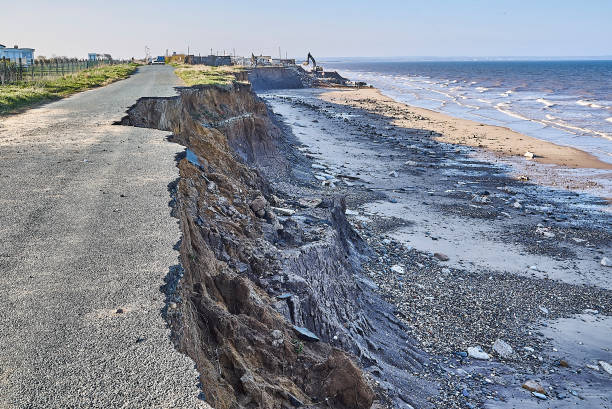
\includegraphics[width = \textwidth]{gravity_erosion.jpg}
\end{textblock*}

\begin{textblock*}{55mm}[0,0](60mm,75mm)
{\footnotesize Marine snow : carbon pump\\
	Estuaries dynamics}\\
\end{textblock*}


%	{%
%		\setlength{\fboxsep}{0pt}%
%		\setlength{\fboxrule}{1pt}%
%		\fbox{\includegraphics[options]{image}}%
%	}%


\end{frame}